
\documentclass{article}
%\documentclass[article]{abntex2}
\usepackage[alf]{abntex2cite}
\usepackage[brazil]{babel}
\usepackage[left=2.5cm,top=2.5cm,right=2.5cm,bottom=2.5cm]{geometry}
\usepackage[utf8]{inputenc}
\usepackage{cancel}
\usepackage{authblk}
\usepackage{graphicx, color}
\usepackage{hyperref}
\usepackage{glossaries}
\usepackage{xifthen} 
\usepackage{tikz}
\usetikzlibrary{arrows}
\usepackage{tikz, tkz-euclide,  pgfplots}
\usepackage{tikzscale}
\usepackage[square,sort,comma,numbers]{natbib}
%[square,sort,comma,numbers]
\usepackage{url}

\makeglossaries
\newacronym{rna}{RNA}{ácido ribunocleico}
\newacronym{dna}{DNA}{ácido desoxirribunocleico}
\newacronym{fiv}{FIV}{vírus da imunodeficiência felina}
\newacronym{hiv}{HIV}{vírus da imunodeficiência humana}
\newacronym{pgl}{PGL}{glicolipídeo fenólico}
\newacronym{aids}{AIDS}{síndrome da imunodeficiência adquirida}
\newacronym{arc}{ARC}{complexo relacionado à AIDS}
\newacronym{si}{SI}{sistema de modelagem suscetível-infectado}


\title{Dinâmica Populacional do Vírus da Imunodeficiência Felina em
Populações de Gatos Domésticos}
\author[1]{Daniel Jacob Tonn}
\author[1]{Nicole dos Santos de Souza}
\affil[1]{Escola de Matemática Aplicada - FGV EMAp, Rio de Janeiro, RJ}
\date{Novembro de 2022}

\begin{document}
\maketitle
\begin{center}
    \textbf{RESUMO}
\end{center}


\noindent Este artigo se dedica à compreensão da circulação do Vírus da Imunodeficiência Felina (FIV), um
retrovírus felino homólogo ao Vírus da Imunodeficiência Humana (HIV), em populações de gatos domésticos. Usando equações diferenciais de primeira ordem com base no modelo SI (Suscetível-Infectado), a dinâmica populacional que será apresentada foi abordada sob duas perspectivas: com e sem transmissão vertical. Como a doença dos felinos não tem cura - e pode comprometer a saúde pública, mesmo que de forma indireta - um modelo epidemiológico que permita entender melhor a sua propagação é de extrema utilidade. Os resultados indicam que a transmissão vertical é extremamente relevante na dinâmica e que, de maneira geral, a situação evoluirá para um equilíbrio estável entre suscetíveis e infectados e não haverá desaparecimento da população ou doença.
\\

\noindent
\text{PALAVRAS-CHAVE: Felinos; Modelo epidemiológico; Retrovírus; Saúde pública; Transmissão.}

%%%%%%%%%%%%%%%%%%%%%%%%%%%%%%%%%%%%%%%%%% GLOSSÁRIOS %%%%%%%%%%%%%%%%%%%%%%%%%%%%%%%%%%
\newpage
% \printglossary[type=\acronymtype]
\printglossary[title ={Lista de Abreviaturas e siglas}]
\newpage

\tableofcontents

\newpage
\section*{INTRODUÇÃO}
\addcontentsline{toc}{section}{INTRODUÇÃO}
Os estudos de circulação da família de vírus  \textit{retroviridae}, popularmente chamados de retrovírus, possuem desfalque quando comparados a trabalhos sobre outros parasitas. De fato, modelar o sistema de propagação de um retrovírus em uma população de mamíferos não é uma tarefa trivial. O período de soropositividade muito longo, bem como a sucessão de diferentes estágios clínicos induzem a necessidade de modelos muito específicos \cite{base}. Além disso, o funcionamento das populações hospedeiras pode ser demasiadamente particular, fazendo com que sua modelagem demande uma boa compreensão dos padrões espaciais e sociais dos hospedeiros.\\

\noindent Neste artigo a questão de interesse é a propagação do \gls{fiv} em gatos domésticos (\textit{Felis Catus}). A doença causada por esse retrovírus compromete o sistema imune do gato de forma parecida com o que o \gls{hiv} faz com seres humanos, por isso é considerado o equivalente da \gls{aids}  para os felinos. Transmitida especialmente de forma horizontal, em geral através de mordidas e arranhões oriundos de disputas territoriais e de fêmeas da espécie,  a \gls{fiv} possui uma frequência maior de casos em machos não castrados com acesso às ruas.\\

\noindent Por se tratar de um lentivírus e ser específico para a espécie, o \gls{fiv} não representa riscos à saúde pública de forma direta. Sabe-se, no entanto, que o animal que contrai a infecção se torna imunossuprimido, correndo o risco de adquirir doenças secundárias como a toxoplasmose e a criptosporidiose ativa que são transmissíveis para humanos. Dessa forma, revela-se uma ameaça para o bem-estar comum - não só dos felinos, mas dos seus tutores\cite{rayane}. \\

\noindent Ademais, uma vez que a imunodeficiência causada pelo retrovírus nos felinos não tem cura, um modelo epidemiológico que permita compreender melhor a propagação da doença - com objetivo de traçar estratégias com relação ao
controle e prevenção da infecção - é indispensável.
Porém, alguns desafios serão encontrados para tal estudo. A população hospedeira que será trabalhada apresenta um alto grau de variabilidade com relação à distribuição geográfica e condições de sobrevivência, bem como questões sociais ligadas aos seus tutores que precisam ser levadas em consideração. Em vista disso, muitos aspectos significativos devem ser omitidos do estudo. Apesar das deficiências, é procurado um modelo que seja capaz de gerar respostas relevantes quanto ao impacto do lentivírus nas populações de gatos, e sobre a influência do funcionamento da população de felinos na propagação do vírus.  \\

\newpage
\section{Revisão Bibliográfica}
\subsection{Hospedeiros e transmissão} 
\subsubsection{Sobre a distribuição geográfica dos hospedeiros}
Com 101,1 milhões de animais domésticos, o Brasil fica em segundo lugar no ranking de maiores criadores de animais domésticos ao redor do mundo, estando atrás apenas dos Estados Unidos que totalizam 146 milhões. A população de gatos no Brasil ocupa cerca de 17,7\%  das residências brasileiras, somando 22 milhões de indivíduos com os números crescendo cada vez mais em virtude da independência, higiene e facilidade de criação \cite{gomes}.\\

\noindent A distribuição geográfica do \gls{fiv} é de caráter mundial, com concentrações em ambientes de maior índice de felinos com comportamento agressivo e menos frequente em regiões de baixa densidade populacional ou localidades em que os gatos domesticados não possuem contato com os felinos de rua. A distribuição das fêmeas se dá especialmente de acordo com a distribuição humana em virtude de fontes alimentícias e para criação dos filhotes, enquanto a distribuição dos machos (pelo menos no período reprodutivo) se dá de acordo com a distribuição das fêmeas receptivas. Os gatos de rua se concentram em grandes áreas onde há fornecimento de algum recurso alimentar. Assim, o padrão de habitação humana é o
principal fator que determina os padrões sociais e
reprodutivos das populações de gatos domésticos.\cite{base}\\

\subsubsection{Sobre a transmissão da doença}
\noindent A doença causada pelo \gls{fiv} é imunossupressora e transmitida especialmente de forma horizontal através de mordidas e arranhões com a troca de sangue e/ou saliva passada de indivíduos infectados para suscetíveis. Entretanto, pode ocorrer de a doença ser propagada também de forma vertical através da amamentação ou via transplacentária. Proporcional ao estágio da doença na mãe, os filhotes podem estar mais ou menos suscetíveis à contaminação. O comportamento agressivo é oriundo normalmente de disputas por alimento, território ou fêmeas da espécie, resultando em uma frequência maior de casos em machos não castrados com acesso às ruas.\\

\noindent O vírus da imunodeficiência felina pertence à família dos \textit{retroviridae}. Na mesma família encontramos o vírus da imunodeficiência humana (\gls{hiv}), que em contraposição ao \gls{fiv}, pode ser transmitido através de relações sexuais.
Além de fornecer um modelo relevante para estudos de \gls{hiv}   , o \gls{fiv} é de particular interesse na ciência veterinária, pois sua infecção dá origem a uma ampla gama de sinais clínicos.
Foi feita uma tentativa de delinear o curso clínico da infecção pelo \gls{fiv} em uma série de cinco estágios análogos aos da infecção pelo \gls{hiv} em humanos. Primeiro, o gato infectado sofre de um estágio agudo que ocorre várias semanas após a infecção e dura de 4 a 16 semanas. Apesar de se recuperar do estágio primário da doença, praticamente todos os gatos infectados com \gls{fiv} se tornam portadores do vírus ao longo da vida. A primeira fase é seguida por uma fase de portador assintomática que dura meses a anos, durante a qual o comportamento do gato não parece ser afetado. Segue-se linfadenopatia generalizada persistente (\gls{pgl}), complexo relacionado à \gls{aids} (\gls{arc}) e a própria \gls{aids}, caracterizada por distúrbios diversos e infecções oportunistas.\cite{base}. Espera-se que a maioria dos gatos infectados morra por "causas naturais" (acidentes rodoviários, caça, envenenamento, etc.) antes de atingir os estágios terminais da infecção por \gls{fiv}. Eles devem ter tempo para transmitir o vírus, mas não para morrer por conta dele. Portanto, esperamos que o vírus tenha um baixo impacto nas populações naturais de gatos domésticos.

\subsection{Trabalhos na área}
Há algumas possibilidades de caminhos a seguir para modelar um problema desse tipo. Em \textit{A diffusive SI model with Allee effect and application to FIV}\cite{difusao}, por exemplo, utiliza-se um \gls{si} de equações diferenciais parciais com a presença do efeito Allee. Em \textit{Dynamics of two feline retroviruses (FIV and FeLV)
within one population of cats} \cite{franck} foi tomada a decisão de modelar a \gls{fiv} em conjunto com outra doença, a Leucemia felina, e verificar sua relação. Já o artigo \textit{"Stochastic dynamics of feline immunodeficiency virus"} \cite{estocastico}, ao contrário dos outros, considera transmissão vertical no modelo e utiliza técnicas de dinâmica estocástica para os cálculos.

\section{Metodologia}
\subsection{O modelo}
O modelo que será utilizado aqui foi embasado nos estudos de Anderson e May \cite{anderson}, descrito em \cite{base} e se trata da dinâmica de uma população de gatos domésticos representada por um conjunto de equações diferenciais de primeira ordem. Considere $N$ como  o número total de gatos no tempo $t$ e $K$ a capacidade máxima de indivíduos no habitat. Assume-se a taxa de crescimento linear da população dada por $r=b-m$, onde $b$ é a taxa de natalidade e $m$ a taxa de mortalidade por causas naturais. A taxa de mortalidade é relacionada linearmente com a proporção de indivíduos e segue a forma $
m+\frac{rN}{K}
$. Com a população livre do \gls{fiv}, a taxa de crescimento da população é dada pela equação logística familiar de Verlhust \cite{helmut}:
\begin{equation} \label{propcres}
\frac{dN}{dt} = rN\left( 1-\frac{N}{K} \right)
\end{equation}

\noindent Para introduzir a doença na população, representa-se $S = S(t)$ para os gatos suscetíveis ao \gls{fiv} e $I = I(t)$ para os gatos infectados, onde $N = S + I$. Para evitar maior complexidade nos cálculos, são considerados todos os estágios (agudo, soropositivo, \gls{pgl}, \gls{arc} e \gls{aids}) como um único. De fato, os três últimos períodos são curtos e implicam na comorbidade do felino, fazendo com que ele esteja distante de disputas de natureza agressiva por território ou acasalamento e também de situações que o levem à morte por causas naturais.

\noindent A transmissão do \gls{fiv} depende diretamente da taxa de encontros entre os animais - a qual será representada pela constante ($\rho$) - da taxa de encontros que resultam em mordidas ou arranhões ($\beta$) e da taxa de eficácia de transmissão dessa doença caso exista contato ($c$). É relativamente simples estimar $c$ através de experimentos em laboratório, mas as taxas $\rho$ e $\beta$ são fortemente influenciadas pela distribuição geográfica dos animais e pelo seus comportamentos. Por conta da complexidade que envolve estimar essas variáveis separadamente, considera-se, para fins de simplificação do modelo, uma constante $\Omega$ que equivale a unificação das três taxas propostas anteriormente ($\rho\beta c$) cuja informação é resumida em taxa de mordidas efetivas para a transmissão do vírus. A taxa de mortalidade pelo \gls{fiv} é independente da densidade populacional e dada por $\alpha$ que corresponde ao inverso do período infeccioso ($\frac{1}{\alpha}$).\\

\noindent Para modelar o processo de transmissão, é preciso que ocorra um encontro entre um indivíduo infectado e um indivíduo suscetível. A proporção de infectados na população é $\frac{I}{I+S}$. Sendo assim, o contágio horizontal pode ser representado da forma:
$$\frac{\rho \beta cSI}{I+S}$$
ou simplesmente 
$$\frac{\Omega SI}{I+S}$$

\noindent Há agora dois caminhos que podem ser seguidos. O artigo base para esse modelo desconsidera a transmissão vertical nos cálculos pois há estudos que contrariam que esse seja um tipo efetivo de propagação da doença, e que os filhotes nascidos de mães infectadas desenvolvem anticorpos contra o \gls{fiv} \cite{vertical}. Porém, há evidências que essa possibilidade de transmissão exista \cite{vertical2}. Portanto, haverá, nesse momento, uma divisão em casos do modelo. Uma das versões irá considerar a transmissão vertical nas equações e a outra irá omitir essa parte. Em ambos os casos, será assumido que não há possibilidade de recuperação (um indivíduo não retorna ao compartimento de suscetíveis uma vez que ingressa em infectados).

\subsubsection{Sem transmissão vertical}
Será tratado aqui o caso em que todos os filhotes nascem suscetíveis (femêas infectadas não transmitem na gestação). Assim, há apenas uma taxa de natalidade considerada = {\it b}. O conjunto de equações diferenciais de primeira ordem
que descreve a dinâmica populacional de gatos domésticos na presença da \gls{fiv} é dada por:

\begin{equation} \label{suscetiveis}
 \frac{dS}{dt}=b(S + I) - mS - \frac{rNS}{K} - \frac{\Omega SI}{N}
\end{equation}

\begin{equation} \label{infectados}
 \frac{dI}{dt}=  \frac{\Omega SI}{N} - mI - \frac{rNI}{K} - \alpha I
\end{equation}

A equação da população total é obtida através da soma da equação~\ref{suscetiveis} com a equação~\ref{infectados}

\begin{equation} \label{poptotal}
\frac{dN}{dt} = rN\left( 1-\frac{N}{K} \right) - \alpha I
\end{equation}

O que corresponde à equação que vimos em ~\ref{propcres} com o acréscimo de uma taxa de mortalidade pela doença.

A representação compartimental pode ser vista na imagem abaixo:

\begin{figure}[!ht]
\centering
%domínio da função
\includegraphics{gráficos/grafo2.tikz}
\end{figure}
 
\subsubsection{Com transmissão vertical}
Fundamentada nos estudos teóricos, a transmissão vertical pode ocorrer na situação que está sendo modelada e será considerada nos cálculos neste caso. Sendo assim, consideraremos que poderá haver recém-nascidos na classe infecciosa. Há a inserção de uma nova constante no modelo ({\it $0 \leq b_1 \leq b$}) que corresponde à taxa de natalidade de gatos infectados ({\it b} é a taxa de natalidade em condições normais, ou seja, sob os gatos suscetíveis). Com isso, a razão $0 \leq \lambda := \frac{b_1}{b} \leq 1$ descreve a proporção de filhotes de fêmeas infectadas que nascem infectados (ou seja, nem toda mãe infectada passará a doença ao seu filhote - fêmeas com \gls{fiv} podem gerar filhotes infectados ou suscetíveis). Nota-se que $\lambda = 0$ indica que não haverá filhotes nascidos infectados - neste caso, não há transmissão vertical. Por sua vez, $\lambda = 1$ significa que todos os filhotes provenientes de mães infectadas nascerão infectados ($b = b_1$).\\


\noindent Dessa forma, o conjunto de equações que representa a dinâmica populacional considerando transmissão vertical é:

\begin{equation} \label{suscetiveis2}
 \frac{dS}{dt}= bS + (b - b_1)I- mS - \frac{rNS}{K} - \frac{\Omega SI}{N}
\end{equation}

\begin{equation} \label{infectados2}
 \frac{dI}{dt}=  b_1I + \frac{\Omega SI}{N} - mI - \frac{rNI}{K} - \alpha I
\end{equation}

\noindent A dinâmica da população total é obtida através da soma da equação~\ref{suscetiveis2} e ~\ref{infectados2} e continua em equilíbrio com o que encontramos através de uma análise sem transmissão vertical. As manipulações estão descritas abaixo:

$$\frac{dS}{dt} + \frac{dI}{dt} = bS + bI - \cancel{b_1I} + \cancel{b_1I} - mS - \frac{rNS}{K} - \cancel{\frac{\Omega SI}{N}} + \cancel{\frac{\Omega SI}{N}} - mI - \frac{rNI}{K} - \alpha I $$
$$\frac{d(S + I)}{dt} = b(S + I) -m(S + I) + rN(-\frac{S}{K} -\frac{I}{K}) - \alpha I $$
$$\frac{dN}{dt} = rN + rN(-\frac{N}{K}) - \alpha I $$
$$\frac{dN}{dt} =  rN(1 -\frac{N}{K}) - \alpha I  $$\\

% \noindent Nota-se que $bS + b_1I$ corresponde à taxa de natalidade total da população, incluíndo infectados e suscetíveis. Por isso, podemos considerar como $bN$ (pois $b$ está relacionada com $r = b- m$ que é o crescimento da população como um todo) e a equação tomará a forma:
% $$ \frac{dN}{dt} = bN - mN + rN(-\frac{N}{K}) - \alpha I $$
% $$ \frac{dN}{dt} = rN(1 - \frac{N}{K}) - \alpha I $$

% coincidindo com a equação final correspondente ao modelo sem transmissão vertical.\\
\noindent O esquema compartimental para ilustrar melhor a dinâmica pode ser visto abaixo:

\begin{figure}[!ht]
\centering
%domínio da função
\includegraphics{gráficos/grafo.tikz}
\end{figure}
\newpage

\subsubsection{Análise dimensional}
Abaixo, exposta em uma tabela, encontra-se a análise dimensional dos modelos. A unidade de tempo ainda não foi caracterizada e os indivíduos são gatos domésticos a serem especificados por  região ou característica futuramente. As lacunas em que a unidade não está informada contém uma constante do modelo, medida ou estimada.
\begin{table}[!h]
    \centering
\begin{tabular}{| l | r | r |}
\hline
Parâmetro & Unidade & Descrição\\
\hline
S = S(t) & indivíduos & quantidade de indivíduos suscetíveis no tempo t\\
I = I(t) & indivíduos & quantidade de indivíduos infectados no tempo t\\
N & indivíduos & quantidade total de indivíduos no tempo t\\
K & indivíduos & capacidade máxima de indivíduos no habitat\\ 
b         & - & constante referente à taxa de nascimentos de indivíduos suscetíveis\\
$b_1$        & - & constante referente à taxa de nascimentos de indivíduos infectados\\
m        & - & contante referente à taxa de mortes por causas naturais\\
r = (b - m) & & constante referente à taxa de crescimento linear da população\\
$\alpha$ & & constante referente à taxa de mortalidade por FIV \\
$\frac{1}{\alpha}$ & unidades de tempo & comprimento do período infeccioso\\
$\rho$ & - & constante referente à taxa de encontros entre os animais\\
$\beta$ & - & constante referente à taxa de encontros que resultam em mordidas/arranhões\\
c & - & constante referente à taxa de eficácia da transmissão do vírus \\
$\Omega = (\rho\beta c)$ & - & contante referente à taxa de mordidas efetivas para transmitir FIV\\
$\lambda = \frac{b_1}{b}$ & - &  proporção de filhotes de fêmeas infectadas que nascem infectados\\
\hline
\end{tabular}
\end{table}

\section{Resultados}
\subsection{Análise de estabilidade}
\subsubsection{Sem transmissão vertical}
Algo a se notar é que quando a taxa de contato efetiva $\Omega$  é menor ou igual à taxa de mortalidade $\alpha$ a quantidade de infectados decresce recorrentemente até atingir o marco de zero infectados, ou seja, a doença deixa de existir pois o fluxo de saída da população infectada é maior que o fluxo de entrada. \cite{base} Por isso, 
$$ 0 \leq \Omega \leq \alpha \implies I(t)\rightarrow 0 \mbox{ quando } t\rightarrow 0.$$
Assumimos, portanto, que $\alpha \leq \Omega$ , seguindo hipóteses biológicas realistas. 
Igualando as equações ~\ref{suscetiveis} e ~\ref{infectados} - ambas em função do tempo - a zero, encontra-se as seguintes soluções de estabilidade:
\begin{itemize}
\item $S=0 \mbox{ e } I=0$;
\item $S=K \mbox{ e } I=0$;
\item $S=\frac{bK(\alpha^2 - \alpha\Omega + b\Omega + \alpha m - \Omega m)}{(\Omega-\alpha)^2(b-m)} \mbox{ e } I=\frac{K(\Omega-\alpha-b)(\alpha^2-\alpha\Omega +b\Omega + \alpha m-\Omega m)}{(\Omega -\alpha)^2(b-m)}$.
\end{itemize}
É importante ver que os dois primeiros equilíbrios citados são triviais e irrelevantes para o estudo da doença. Enquanto o primeiro equilíbrio se refere a inexistência de população, o segundo é referente a uma população livre da doença, tendendo à capacidade de suporte do habitat. O último equilíbrio, por sua vez  - que deve ser estritamente positivo - não é trivial e pode ser encontrado através de programas computacionais.\\

\noindent Na figura abaixo está presente a plotagem do comportamento do \gls{fiv} sem transmissão vertical para os valores de parâmetros $b=2.4,K=46,\alpha=0.2, \Omega=3 \mbox{ e } m=0.6$ - as estimações foram retiradas dos estudos de campo do artigo base e têm significado biológico. Veja que, para qualquer que seja a população inicial, ao restringir a quantidade de infectados sendo positiva, atinge-se o terceiro ponto de equilíbrio em discussão.

\begin{figure}
    \centering
    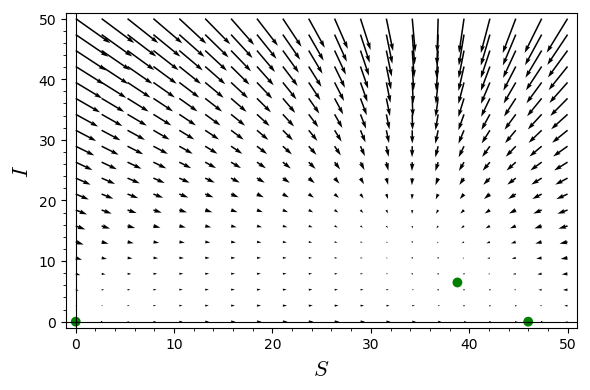
\includegraphics[width=14cm]{imagens/plot1-biologia.PNG}
    \caption{Equilíbrio populacional sem transmissão vertical}
    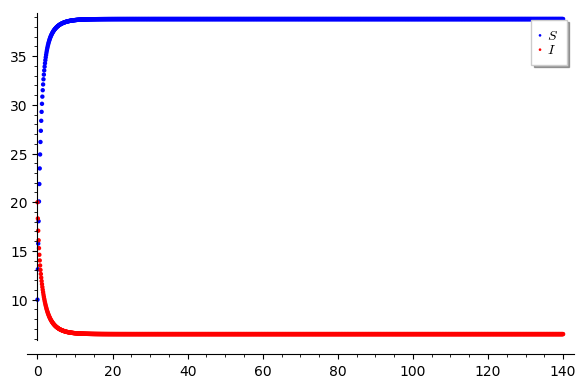
\includegraphics[width=14cm]{imagens/curvasemtransmissaovertical.png}
    \caption{Convergência numérica sem transmissao vertical}
    \label{fig:my_label}
\end{figure}

\subsubsection{Com transmissão vertical}
No caso atual, a análise entre $\Omega$ e $\alpha$ sofre influência de uma terceira constante $b_1$ inserida no modelo, que é a proporção de nascidos sadios de mães infectadas. Se  $ (\Omega +(b- b_1)) \leq \alpha $, a doença tende a desaparecer, ou seja:
$$ 0 \leq (\Omega +(b- b_1)) \leq \alpha \implies I(t)\rightarrow 0 \mbox{ quando } t\rightarrow 0.$$
Assumimos, portanto, que $ \alpha \leq (\Omega +(b- b_1))  $. Igualando as equações ~\ref{suscetiveis2} e ~\ref{infectados2} a zero, encontra-se as soluções de estabilidade:

%e a zero e definindo como em \textit{i)} $b_1=0$,%
\begin{itemize}
\item $S=0 \mbox{ e } I=0$;
\item $S=K \mbox{ e } I=0$.
\item $S=\frac{K\alpha b_1^2-Kb_1m(\Omega-\alpha) -Kb_1(\Omega\alpha - \alpha^2-b(\Omega-\alpha)   )  }{(\Omega^2-2\Omega\alpha+\alpha^2)(b-m)} \mbox{ e }\\ I=\frac{K[\Omega^2\alpha-2\Omega\alpha^2+\alpha^3+\alpha b_1^2-b(\Omega^2-2\Omega\alpha+\alpha^2)-b_1(2\Omega\alpha-2\alpha
^2 -b(\Omega-\alpha))+m(\Omega^2-2\Omega\alpha+\alpha^2-b_1(\Omega-\alpha)]}{(\Omega^2-2\Omega\alpha+\alpha^2)(b-m)}$;
\end{itemize}

\noindent Quando consideramos uma taxa positiva de transmissão vertical da doença, temos dois casos a avaliar: \textit{i}) todos os filhotes da ninhada serão infectados; \textit{ii}) uma parte da ninhada nascerá infectada e a outra parte nascerá sadia.\\

\noindent Nossa primeira análise será considerando o caso (i) $b_1 = 0$. Observe as figuras abaixo:

\begin{figure}[!h]
    \centering
     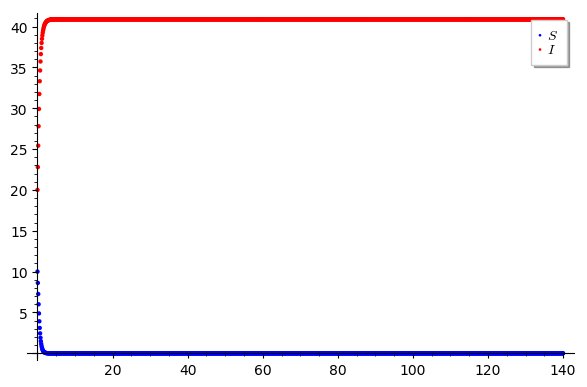
\includegraphics[width=14cm]{imagens/b1zerocurvas.png}
    \caption{Convergência numérica para $b_1=0$}
    \label{fig:my_label}
\end{figure}

\begin{figure}[!h]
    \centering
     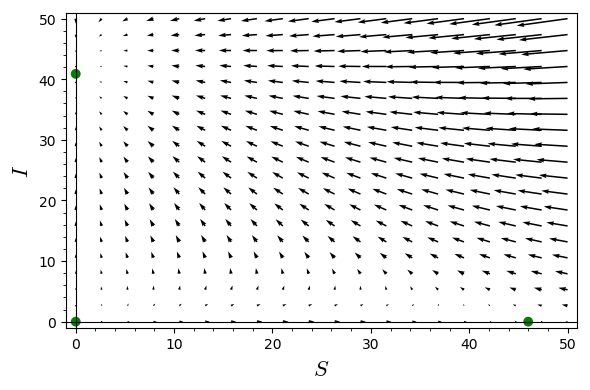
\includegraphics[width=14cm]{imagens/plot2-biologia.PNG}
    \caption{Diagrama de fase com $b_1=0$}
    \label{fig:my_label}
\end{figure}
    
\newpage
\noindent Note que, se $b_1=0$, todas as soluções estão sobre algum dos eixos. Portanto, se a população inicial contiver uma quantidade não nula de indivíduos infectados, a tendência é que toda a população venha a ser completamente infectada. No caso contrário, em que não existem indivíduos infectados, o equilíbrio é justamente a capacidade suporte do habitat.\\
% Na figura abaixo está presente a dinâmica populacional com transmissão vertical para os parâmetros estimados $b = 2.4,b_1=0, K = 46, α = 0.2, Ω = 3 \mbox{ e } m = 0.6$. É observável que qualquer que seja a população inicial restringindo a quantidade de infectados a ser positiva atinge o terceiro ponto de equilíbrio.%

\noindent Por outro lado, em \textit{(ii)}, quando $b_1>0$, a situação é diferente. Veja:

\begin{figure}[!h]
    \centering
     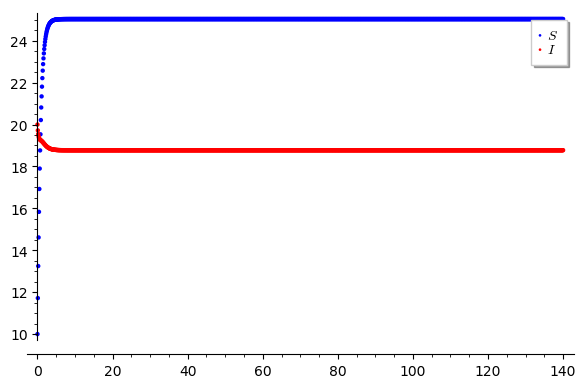
\includegraphics[width=14cm]{imagens/b1mzc.png}
    \caption{Convergência numérica para $b_1>0$}
    \label{fig:my_label}
\end{figure}

\begin{figure}[!h]
    \centering
      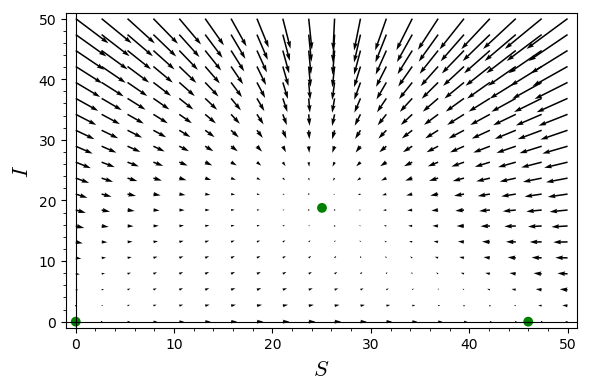
\includegraphics[width=14cm]{imagens/b1mzs.png}
    \caption{Diagrama de fase com $b_1>0$}
    \label{fig:my_label}
\end{figure}
    
\newpage
\noindent Para os parâmetros $b = 2.4,b_1=1.6, K = 46, α = 0.2, Ω = 3 \mbox{ e } m = 0.6$, encontramos um ponto de equilíbrio não trivial com uma proporção positiva de indivíduos suscetíveis e outra positiva de infectados. Pelo diagrama de fase, é visível que quaisquer que seja a população inicial de infectados maior que zero, a convergência tende ao ponto de equilíbrio não trivial. No caso em que não existem infectados, a convergência é justamente para a capacidade máxima do habitat. Além disso, alguns testes foram realizados alterando o valor escolhido para $b_1$, e observou-se que, quanto mais próximo de 0, mais próximo o 3° ponto de equilíbrio fica dos eixos (a população suscetível vai para K ou se extingue), enquanto o contrário faz o 3° ponto tender ao equilíbrio sem transmissão vertical (equilíbrio com número de suscetíveis próximo de K).

\newpage
\section{Discussão}
\subsection{Sem transmissão vertical}
Conforme os cálculos realizados, temos que, quando não há transmissão vertical e o FIV é introduzido em uma população de gatos, a infecção inevitavelmente se desenvolve e é mantida. A presença do vírus na população, então, não conduz à extinção de gatos suscetíveis ou infectados, mas a um estágio de equilíbrio estável de ambas as categorias, em proporções dependentes de parâmetros específicos da população. Os parâmetros que foram utilizados para essa modelagem são provenientes do artigo base já citado que trabalhou com conhecimento empírico. \\

\noindent É possível observar que, no equilíbrio não trivial, foi obtida uma quantidade de suscetíveis muito próxima da capacidade suporte do habitat. Isso indica que o impacto do vírus, em termos de redução do
tamanho da população em equilíbrio, não é tão significativo. Esse fato parece ainda mais intuitivo ao comparar expectativa de vida com a duração da infecção.

\subsection{Com transmissão vertical}
Para uma modelagem sob outra perspectiva, foi introduzida uma nova característica no modelo: fêmeas infectadas podem gerar filhotes infectados ou suscetíveis. Para isso, o foco da análise ficou sob uma nova variável ($b_1$), referente a taxa de natalidade de gatos infectados. Vimos que, se $b_1 = 0$, não há transmissão vertical e assim o modelo retorna ao caso anterior. No caso $b_1 = b$, onde todos os filhotes provenientes de mães infectadas nascerão com a doença, não obtém-se equilíbrios não-triviais - ou seja, haverá o desaparecimento da doença ou da população. Para $0 < b_1 < b$, por sua vez, obtemos um equilíbrio estável entre os dois compartimentos da população. O equilíbrio vai se aproximar ou desaproximar dos dois primeiros casos conforme $b_1$ é alterado.  


\newpage
\section{Conclusão}
Com base na análise realizada, conclui-se que, a não ser que se tenha certeza de que todos os filhotes de uma mãe infectada nascerão infectados, a dinâmica evoluirá para um equilíbrio estável com quantidades positivas de suscetíveis e infectados. Isso indica que a doença não causará a extinção da população, mas estará presente entre os indivíduos inevitavelmente, uma vez que inserida. Esse fato é apoiado teoricamente, já que há indícios da \gls{fiv}e permanência dela nas mais diversas populações de gatos domésticos - até mesmo em ilhas.\\

\noindent Além disso, foi visto que, na ausência de transmissão vertical, o número de indivíduos no compartimento dos suscetíveis em equilíbrio é muito próximo do limite do habitat. Isso mostra que a doença não é tão contagiosa e não terá um impacto tão significativo sob a população - conforme era esperado. Por outro lado, com taxas altas de transmissão vertical, a dinâmica da doença tende a infectar a população como um todo - mesmo nesse caso, é mais provável que os gatos venham a óbito por causas naturais do que por \gls{FIV}, por conta do período de infecção muito longo que permite que eles transmitam a doença por muito tempo mas não morram por ela. Mesmo assim, a transmissão vertical tem muita relevância no modelo e deve ser mantida em posição de observação com relação a saúde pública.\\

\noindent Outro ponto que precisa ser levado em consideração é que a taxa de transmissão deve variar muito de acordo com a população hospedeira. Os parâmetros que foram usados são provenientes de estudos com populações de gatos domésticos em áreas rurais - o que deve, intuitivamente, ser menor se comparado com populações de gatos de rua em áreas urbanas, por exemplo (em vista de que disputas por território e alimento são mais recorrentes).\\

\noindent Para um diagnóstico mais preciso, seria interessante utilizar de dados reais para estimar os parâmetros de diferentes formas e com variabilidade de populações hospedeiras (com relação a cultura, geografia, entre outros fatores). O impasse nesse quesito é que a coleta de dados precisaria ser feita por um longo período de tempo para uma análise mais profunda, o que é muito pouco viável.\\

\noindent Em suma, deve-se frisar que esse modelo é muito mais voltado a conceituação dos mecanismos de
transmissão do FIV do que previsões ou estimativas precisas de parâmetros. 
\newpage
\bibliography{bibliografia/ref.bib}
\end{document}
